%%% Preamble
\documentclass[DIV=calc,paper=a4,fontsize=11pt,twocolumn]{scrartcl}

\usepackage{lipsum}                                                 
\usepackage[utf8x]{inputenc}
\usepackage[english]{babel}								% English language/hyphenation
\usepackage[protrusion=true,expansion=true]{microtype}	% Better typography
\usepackage{amsmath,amsfonts,amsthm}					% Math packages
\usepackage[pdftex]{graphicx}							% Enable pdflatex
\usepackage[svgnames]{xcolor}							% Enabling colors by their 'svgnames'
\usepackage[hang, small,labelfont=bf,up,textfont=it,up]{caption}	% Custom captions under/above floats
\usepackage{epstopdf}									% Converts .eps to .pdf
\usepackage{subfig}										% Subfigures
\usepackage{booktabs}									% Nicer tables
\usepackage{fix-cm}										% Custom fontsizes
\usepackage{csquotes}
\usepackage[authoryear,round]{natbib}
\usepackage{float}
\bibliographystyle{natdin}



%%% Custom sectioning (sectsty package)
\usepackage{sectsty}									% Custom sectioning (see below)
\allsectionsfont{\usefont{OT1}{phv}{b}{n}}				% Change font of al section commands
														% bch-b-n: CharterBT-Bold font

\sectionfont{\usefont{OT1}{phv}{b}{n}}					% Change font of \section command
														% bch-b-n: CharterBT-Bold font

%%% Headers and footers
\usepackage{fancyhdr}									% Needed to define custom headers/footers
    \pagestyle{fancy}									% Enabling the custom headers/footers
\usepackage{lastpage}   

% Header (empty)
\lhead{}
\chead{}
\rhead{}
% Footer (you may change this to your own needs)
\lfoot{\footnotesize 2013 \textbullet ~ Here the Title again}
\cfoot{}
\rfoot{\footnotesize page \thepage\ of \pageref{LastPage}}  % "Page 1 of 2"
\renewcommand{\headrulewidth}{0.0pt}
\renewcommand{\footrulewidth}{0.4pt}



%%% Creating an initial of the very first character of the content
\usepackage{lettrine}
\newcommand{\initial}[1]{%
     \lettrine[lines=3,lhang=0.3,nindent=0em]{
                    \color{DarkGoldenrod}
                    {\textsf{#1}}}{}}



%%% Title, author and date metadata
\usepackage{titling}										% For custom titles

\newcommand{\HorRule}{\color{DarkGoldenrod}\rule{\linewidth}{1pt}}

\pretitle{\vspace{-30pt} \begin{flushleft} \HorRule \fontsize{35}{35} \usefont{OT1}{phv}{b}{n} \color{DarkRed} \selectfont }
\title{Here the title of my document}					% Title of your article goes here
\posttitle{\par\end{flushleft}\vskip 0.5em}

\preauthor{\begin{flushleft} \large \lineskip 0.5em \usefont{OT1}{phv}{b}{sl} \color{DarkRed}}
\author{Steffen Tröster \\}											% Author name goes here
\postauthor{\footnotesize \usefont{OT1}{phv}{m}{sl} \color{Black} 
                    University of Tampere, 2013							% Institution of author
                    \par\end{flushleft}\HorRule}

\date{}																% No date



%%% Begin document
\begin{document}
\maketitle
\thispagestyle{fancy}		% Enabling the custom headers/footers for the first page 
% The first character should be within \initial{}
\initial{O}\textbf{pen-source software development can be divided into several phases. The phases specified here are derived from Sharma et al. \citep{ZitovaF03}}

\section{Introduction}

The open source software development paradigm is one of the most upcoming way of new software development. Software developed in this way is free in use, spreading and contribution with the condition of continuing the open source paradigm. But this "free" results out of open source development processes are nearly all commercial projects with service opportunities \citep{Wheeler}.

To ensure a proper result in open source development with all different co-developer, from an established community, there should be a sharp regulation progress for input and iterations. Also difficult is the opportunity to develop from everywhere in the world. Therefor the open source development paradigm uses a set of different software engineering tools with features which helps the given in cases like collaboration, status-tracking and testing.

\enquote{To a large extent, the open source culture and methodology are conveyed to new developers via the toolset itself, and through the demonstrated usage of these tools on existing projects.} \citep{Robbins02adoptingoss}

\subsection{Open Source Software Development Model}

Next to the given toolset, there is an Open Source Development Model which is characterized by processes and values of a different kind as traditional proprietary development models. This model takes a new approach for more fluidly development by increasing collaboration, continuous integration and testing. It also involves the end-users deeper into design decisions. Some companies may use a slightly modified version of this model depending on their claims. \citep{Haddad11}

The Model in Figure \ref{fig:feature-life-cycle} shows a typical feature life-cycle. A feature request is coming from the user or developer community of the project by mailing list or issue tracker. It will discussed in the whole community and results to an architecture or design decision which is received into to implementation process if it is accepted. The new feature will after the implementation verified by continuous integration and (automated) testing. This whole process is iteration based and can flow back to the decision process to ensure a necessary project quality when for example a testing of a feature failed and when it contradicts other design decisions. After a successfully testing the feature will be deployed in a new project version and can be maintenanced by the user and development community. \citep{Haddad11}

\begin{figure*}[ht]
    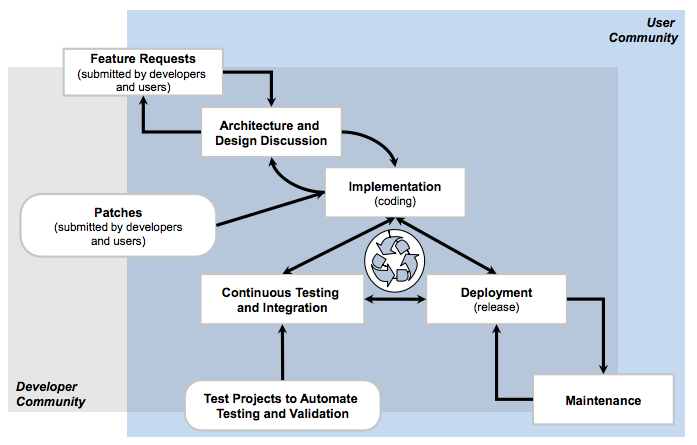
\includegraphics[width=0.9\textwidth ]{img/feature-life-cycle.png}{}
    \centering
    \caption{Feature life-cycle in the open source development model. \citet{Haddad11}}\label{fig:feature-life-cycle}
\end{figure*}

\section{Tools in Open Source Software Development}

Software Engineering tools which are created and used in open source software development are fitting to the different processes of the given software development model. These tools are widly the result of daily practices so that they carry support for the given use cases in open source software development. \citep{Robbins02adoptingoss} 

Back to the model of \citet{Haddad11}, each process is constituting a special type of tool. First of all communication tools are important to contribute feature requests, issues and bugs to a project. These tools are also used to make the design decisions in the developer and user community. The second topic of tools are version control systems and collaboration tools to facilitate parallel contribution from all over the world. The software need to be tested according to the given open source model after contribution. Therefor a toolset of different testing and continues integration tools are available. They will be discussed in the following sub chapters.

\subsection{Communication - Issue and Bugtracking}
\subsection{Version Control and Collaboration}
\subsection{Testing and Continues Integration}
\subsubsection{Testing Methods}



\bibliography{library}

\end{document}
